\documentclass{beamer}
\usepackage[document]{ragged2e}
\usepackage[spanish]{babel}
\usepackage[utf8]{inputenc}
\usepackage{lmodern}
\usepackage{amsmath}
\mode<presentation> {
	%\usetheme{default} % liso sin nada bueno simple
	%\usetheme{Pittsburgh} % liso sin nada bueno simple
	%\usetheme{Montpellier} % liso con orden arriba
	%\usetheme{Singapore} % orden arriba liso (mas oscuro)
	%\usetheme{Boadilla} % parecido al liso, con pie de pagina
	
	%\usetheme{Luebeck} % encabezado y pie de pagina (oscuro)
	%\usetheme{Copenhagen} % encabezado y pie de pagina
	\usetheme{Madrid} % encabezado y pie de pagina (azul)
		
	%\usetheme{Goettingen} % con orden a la derecha
	%\usetheme{Marburg} % con orden a la derecha (Oscuro)
	%\usetheme{Hannover} % con orden a la izquierda
	
	%%%%% Colores %%%%%
	%\usecolortheme{albatross} % fondo azul
	%\usecolortheme{beetle} % fondo plomo
		
	%\usecolortheme{dove} % quita todo el color, blanco
	%\usecolortheme{fly} % todo plomo

	%\usecolortheme{crane} % encabezado pie de pagina, naranjo
	%\usecolortheme{seagull} % encabezado pie de pagina, plomo
	\usecolortheme{seahorse} % encabezado pie de pagina azulplomo
	%\usecolortheme{wolverine} % encabezado pie de pagina, amarillo
}
\usepackage{graphicx}
\usepackage{subfigure}
%----------------------------------------------------------------------------------------
%	TITLE PAGE
%----------------------------------------------------------------------------------------

\title[Econometr\'ia Financiera]{Econometr\'ia Financiera}
\subtitle{2023\\
Programa y Unidad I}
\author[Rodrigo Ortiz] {Rodrigo Ortiz}
\institute[UAH]{
	Universidad Adolfo Ib\'a\~nez \\
}
\date{Chile, 2023}
%---------------------------------------------------------
% Presentaci�n
%---------------------------------------------------------
\begin{document}
\begin{frame}
	\titlepage
\end{frame}
%---------------------------------------------------------
% Indice
%---------------------------------------------------------
\begin{frame}
	\frametitle{Planificaci\'on}
	\framesubtitle{Agenda}
	\tableofcontents
\end{frame}

\section{Introducci\'on}
\begin{frame}
\frametitle{Introducci\'on}

El objetivo de este curso es introducir al alumno a las propiedades de los modelos de series de tiempo, as\'i como a las aplicaciones emp\'iricas. Al final del curso, el alumno deber\'a ser capaz de identificar las herramientas m\'as apropiadas para abordar un problema financiero de car\'acter estad\'istico.

\vspace{0.5cm}
El curso se estructurar\'a de manera tal que el alumno se vea expuesto a la teor\'ia y a su aplicaci\'on, utilizando para tal fin programas estad\'isticos de uso amplio, tales como STATA y R-Project.

\end{frame}

\begin{frame}
\frametitle{Objetivos del curso}

Al finalizar el curso se espera que cada participante sea capaz de:

\begin{itemize}
  \item Conocer y aplicar herramientas estad\'isticas de descripci\'on de datos.
  \item Identificar las herramientas econom\'etricas de series de tiempo m\'as apropiadas para abordar un problema financiero.
  \item Utilizar con destreza un paquete econom\'etrico, tal como STATA y R-Project.
\end{itemize}
\end{frame}

%--------------------------------------------------------
% Evaluaciones y aprobaci�n
%--------------------------------------------------------
\section{Evaluaciones}
\begin{frame}
\frametitle{Evaluaciones}

\begin{itemize}	
    \item 1 prueba (40\%)
    \item 1 trabajo grupal (30\%)
    \item 1 examen (30\%)
\end{itemize}

Importante:

\begin{itemize}
    \item No se elimina ninguna nota.
    \item A fin de facilitar la correcci\'on, las gu\'ias y el trabajo se deben realizar en grupos de 4-5 alumnos. No se aceptar\'an entregas individuales.
    \item Se recuerda que, por reglamento, el alumno debe contar con una asistencia de, al menos, un 75\%.
\end{itemize}

\end{frame}


%--------------------------------------------------------
% Bibliograf�a
%--------------------------------------------------------
\section{Bibliograf\'ia: Esencial}

\begin{frame}
\frametitle{Bibliograf\'ia: Esencial}

\begin{itemize}
  \item Brooks, C. (2014). Introductory Econometrics for Finance. Tercera edici\'on. Cambridge University Press.
  \item Fabozzi, F, S. Focardi, S. Rachev \& B. Arshanapalli (2014). The Basics of Financial Econometrics: Tools, Concepts and Asset Management Applications. Wiley.
  \item Gonz\'alez-Rivera, G (2012). Forecasting for Economics and Business. Primera edici\'on. Routledge.
  \item Hanke, J. \& D. Wichern (2010). Pron\'osticos en los negocios. Novena edici\'on. Pearson.
  \item Newbold, P., W. Carlson, \& B. Thorne (2013). Estad\'istica para administraci\'on y econom\'ia. Octava edici\'on. Pearson.
  \item Novales, A. (1993). Econometr\'ia. Segunda edici\'on. McGraw-Hill.
  \item Walpole. R., R. Myers, S. Myers, K. Ye (2012). Probabilidad y estad\'isticas para ingenier\'ia y ciencias. Novena edici\'on. Pearson.
  \item Wooldridge, J. (2015). Introducci\'on a la Econometr\'ia. Quinta edici\'on. Cengage Learning.
\end{itemize}

\end{frame}


\section{Bibliograf\'ia: Avanzada}

\begin{frame}
\frametitle{Bibliograf\'ia: Avanzada}

\begin{itemize}
  \item Enders, W. (2015). Applied Econometric Times Series. Cuarta edici\'on. Wiley Series in Probability and Statistics.
  \item Mills, T. and Markelos, R. (2008). The Econometric Modelling of Financial Time Series. Cambridge University Press.
\end{itemize}

\end{frame}
%--------------------------------------------------------
% Contenidos clase de hoy
%--------------------------------------------------------
\section{Repaso}
\subsection{Tipos de Variables}
\begin{frame}
\frametitle{Tipos de Variables}

\begin{itemize}
\item Variables cuantitativas: edad, estatura, renta
	\begin{itemize}
	\item Continuas o de intervalo (estatura)
	\item Discretas (n\'umero de hermanos)
	\end{itemize}
\item Variables cualitativas, atributo o categor\'ia: color, g\'enero, municipio de nacimiento
	\begin{itemize}
	\item Binarias, dos valores disponibles (g\'enero, se convierte en num\'erica)
	\item Generales (color de ojos, podemos transformarlas en binarias)
	\end{itemize}
\end{itemize}
\end{frame}


\begin{frame}
\frametitle{Tipos de Variables}

\begin{itemize}
\item Variables cualitativas, atributo o categor\'ia:
\item Tenemos $p$ variables num\'ericas en un conjunto de $n$ elementos.
\item Cada una de estas $p$ variables se denomina una variable {\bf escalar o univariante}.
\item El conjunto de $p$ variables forman una variable {\bf vectorial o multivariante}
\begin{center}
 $X = \begin{bmatrix}
                x_{11} & x_{12} & \ldots & x_{1p} \\
                x_{21} & x_{22} & \ldots & x_{2p} \\
                \vdots &\vdots & \ddots & \vdots \\
                x_{n1} & x_{n2} & \ldots & x_{np} \end{bmatrix}$
\end{center}
\item $p$ variables escalares en cada uno de los $n$ elementos pueden representarse en una matriz $X$, de dimensiones $(n,p)$, la {\bf matriz de datos}.
\end{itemize}
\end{frame}

\subsection{An\'alisis Univariante}
\begin{frame}
\frametitle{An\'alisis univariante}

La variable escalar $x_j$, la media muestral

\begin{align*}
\overline{x}&=\frac{1}{n}\sum_{i=1}^{n}{x_{ij}}
\end{align*}

que para una variable binaria es la frecuencia relativa de aparici\'on del atributo y para una num\'erica es el centro de gravedad o geom\'etrico de los datos.

Medida de variabilidad con relaci\'on a la media, la {\bf desviaci\'on t\'ipica muestral}

\begin{align*}
s_j&=\sqrt{\frac{1}{n}\sum_{i=1}^{n}{d_{ij}}}=\sqrt{\frac{1}{n}\sum_{i=1}^{n}{(x_{ij}-\overline{x})^2}}
\end{align*}

\end{frame}


\begin{frame}
\frametitle{An\'alisis univariante}
El cuadrado de la desviaci\'on t\'ipica, la {\bf varianza muestral}

\begin{align*}
s_j^2&=\frac{1}{n}\sum_{i=1}^{n}{dij}=\frac{1}{n}\sum_{i=1}^{n}{(x_{ij}-\overline{x})^2}
\end{align*}

Relaci\'on lineal entre dos variables, la {\bf covarianza muestral} entre $x_j$ y $x_k$

\begin{align*}
s_{jk}&=\frac{1}{n}\sum_{i=1}^{n}{(x_{ij}-\overline{x_{j}})(x_{ij}-\overline{x_{k}})}
\end{align*}
\end{frame}


\begin{frame}
\frametitle{An\'alisis univariante}
Medida de relaci\'on lineal entre $x_j$ y $x_k$, el {\bf coeficiente de correlaci\'on muestral}

\begin{align*}
r_{jk}&=\frac{s_{jk}}{\sqrt{s_{jj}}\sqrt{s_{kk}}}=\frac{\sum_{i=1}^{n}{(x_{ij}-\overline{x_j})(x_{ik}-\overline{x_k})}}{\sqrt{\sum_{i=1}^{n}{(x_{ij}-\overline{x_j})^2}}{\sqrt{\sum_{i=1}^{n}{(x_{ik}-\overline{x_k})^2}}}}\\
& -1\leq r \leq 1
\end{align*}

{\bf Coeficiente de variaci\'on}: magnitud del error promedio de medici\'on como porcentaje de la cantidad medida.
\begin{align*}
CV_j&=\sqrt{\frac{s_j^2}{\overline{x_j}^2}}
\end{align*}
\end{frame}

\begin{frame}
\frametitle{An\'alisis univariante}
{\bf Coeficiente de asimetr\'ia}

\begin{align*}
A_j&=\frac{1}{n}\sum_{i=1}^{n}{\frac{(x_{ij}-\overline{x_j})^3}{s_j^3}}
\end{align*}

{\bf Coeficiente de homogeneidad}: mide la relaci\'on entre la variabilidad de las desviaciones y la desviaci\'on media
\begin{align*}
H_j&=\frac{\frac{1}{n}\sum_{i=1}^{n}{(d_{ij}-s_j^2)^2}}{s_j^4}\geq 0
\end{align*}
\end{frame}

\begin{frame}
\frametitle{An\'alisis univariante}
{\bf Coeficiente de kurtosis}: Mide la relaci\'on entre la variabilidad de las desviaciones y la desviaci\'on media.

\begin{align*}
K_j&=\frac{1}{n}\sum_{i=1}^{n}{\frac{(x_{ij}-\overline{x_j})^4}{s_j^4}}
\end{align*}
\end{frame}

\subsection{Modelo de Regresi\'on Lineal M\'ultiple}
\begin{frame}
    \frametitle{Modelo de Regresi\'on Lineal M\'ultiple}

\begin{itemize}
\item $x_k$: variables predictoras o independientes, $k=1,\dots,p$
\item $y$: variable respuesta o dependiente
\item $n$: observaciones independientes de $y$
\item $\beta_k$ coeficientes de regresi\'on, {\bf efecto marginal} (cambio esperado) en $y$ por cambio unitario en $x_k$ cuando el resto de las variables permanece constante
\item $\epsilon$: {\bf efecto} de todas las variables no incluidas en el an\'alisis
\end{itemize}

\end{frame}

\begin{frame}
\frametitle{Modelo de Regresi\'on Lineal M\'ultiple}
\framesubtitle{Modelo matem\'atico}

\begin{align*}
y_1&=\beta_0+\beta_1x_{11}+\beta_2x_{12}+\dots+\beta_px_{1p}+\epsilon_1\\
y_2&=\beta_0+\beta_1x_{21}+\beta_2x_{22}+\dots+\beta_px_{2p}+\epsilon_2\\
\vdots & \\
y_n&=\beta_0+\beta_1x_{n1}+\beta_2x_{n2}+\dots+\beta_px_{np}+\epsilon_n
\end{align*}

\begin{center}

$X = \begin{bmatrix}
                y_{1} \\
                y_{2} \\
                \vdots \\
                y_{n}
                \end{bmatrix}
                 = \begin{bmatrix}
                1 & x_{11} & x_{12} & \ldots & x_{1p} \\
                1 & x_{21} & x_{22} & \ldots & x_{2p} \\
                \vdots &\vdots & \ddots & \vdots \\
                1 & x_{n1} & x_{n2} & \ldots & x_{np} \end{bmatrix}
                \begin{bmatrix}
                \beta_{0} \\
                \beta_{1} \\
                \vdots \\
                \beta_{p}
                \end{bmatrix}
                +
                 \begin{bmatrix}
                \epsilon_{0} \\
                \epsilon_{1} \\
                \vdots \\
                \epsilon_{p}
                \end{bmatrix}
                $
\end{center}

\begin{align*}
y_{(nx1)}=X_{(nx(p+1))}\beta_{((p+1)x1)}+\epsilon_{(nx1)}
\end{align*}
\end{frame}


\begin{frame}
\frametitle{Modelo de Regresi\'on Lineal M\'ultiple}
\framesubtitle{Modelo matem\'atico - Supuestos}

\begin{align*}
y_{(nx1)}=X_{(nx(p+1))}\beta_{((p+1)x1)}+\epsilon_{(nx1)}
\end{align*}

\begin{itemize}
\item E($\epsilon$)=$0_{nx1}$
\item var($\epsilon$)=E($\epsilon$$\epsilon$')
\item cov($\epsilon_j$,$\epsilon_k$)=E($\epsilon_j$$\epsilon_k$')=0 (independientes entre s\'i)
\item $\epsilon$$\sim NM_{m} (0,\sigma^2 I_n)$
\item $\beta$ y $\sigma^2$ {\bf son par\'ametros desconocidos}
\end{itemize}
\end{frame}



\begin{frame}
\frametitle{Modelo de Regresi\'on Lineal M\'ultiple}

Tenemos $p+1$ par\'ametros $\beta$ y $\sigma^2$. Necesitamos m\'as datos que los par\'ametros a estimar. Hip\'oyesis adicionales:

\begin{itemize}
\item N\'umero m\'inimo de observaciones igual a $p+1$
\item Variables $x_k$ linealmente independientes
\item Para cada conjunto fijo de valores de $x_k$, la distribuci\'on de {\bf y} tiene media $E[{\bf y}]=\beta_0+\beta_1x_1+\dots+\beta_px_p$
\item Media como funci\'on {\bf lineal} de los par\'ametros no conocidos $\beta_o,\beta_1,\dots,\beta_p$
\item $var({\bf y})$ es constante, no depende de los valores de $x_k$
\item La variable respuesta {\bf y}$\sim N ({\bf X}\beta,\sigma^2 I_n)$
\end{itemize}
\end{frame}

\subsection{Estimaci\'on por M\'inimos Cuadrados Ordianarios}

\begin{frame}
\frametitle{Estimaci\'on por M\'inimos Cuadrados Ordinarios}

{\bf X} rango m\'aximo $p+1\leq n$. Se desea encontrar $\beta$ tal que se minimice la diferencia.

\begin{align*}
L=&\sum_{i=1}^n{(y_i-\beta_0-\beta_1x_{i1}-\dots-\beta_px_{ip})}\\
&=\sum_{i=1}^n{\epsilon_i^2}\\
&=\epsilon'\epsilon\\
&= ({\bf y}-{\bf X}\beta)'({\bf y}-{\bf X}\beta)\\
&={\bf y'y}-{\bf y'X}\beta-\beta'{\bf X'y}+\beta'{\bf X'X}\beta\\
&={\bf y'y}-2\beta'{\bf X'y}+\beta'{\bf X'X}\beta
\end{align*}
\end{frame}


\begin{frame}
\frametitle{Estimaci\'on por M\'inimos Cuadrados Ordinarios}

\begin{align*}
\frac{\partial L}{\partial \beta}|_{\widehat{\beta}}&=-2{\bf X'y}+2{\bf X'X}\\
{\bf X'X}\widehat{\beta}&={\bf X'}y
\end{align*}

El {\bf estimador de m\'inimos cuadrados de} $\beta$ es
\begin{center}
$\widehat{\beta}=({\bf X'X})^{-1}{\bf X'y}$
\end{center}

El {\bf modelo de regresi\'on ajustado} es:
\begin{center}
$\widehat{\bf y}={\bf X}\widehat{\beta}$
\end{center}

$\widehat{\beta}$ es el estimador lineal insesgado de m\'inima varianza.
\end{frame}

\begin{frame}
\frametitle{Estimaci\'on por M\'inimos Cuadrados Ordinarios}
\framesubtitle{Ajuste del modelo de regresi\'on m\'ultiple}

\begin{align*}
SC_T&=SC_R+SC_E\\
\sum_{i=1}^n{(y_i-\overline{y})^2}&=\sum_{i=1}^n{(\widehat{y_i}-\overline{y})^2}+\sum_{i=1}^n{(y_i-\widehat{y_i})^2}
\end{align*}

   \begin{figure}
   \begin{center}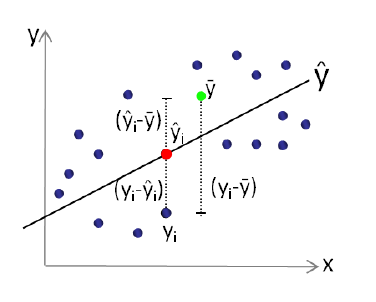
\includegraphics[width=6cm]{var.png}\end{center}
   \end{figure}

\end{frame}


\begin{frame}
\frametitle{Estimaci\'on por M\'inimos Cuadrados Ordinarios}
\framesubtitle{Coeficiente de determinaci\'on}

\begin{align*}
SC_T&=SC_R+SC_E\\
\sum_{i=1}^n{(y_i-\overline{y})^2}&=\sum_{i=1}^n{(\widehat{y_i}-\overline{y})^2}+\sum_{i=1}^n{(y_i-\widehat{y_i})^2}
\end{align*}

\begin{align*}
R^2&=1-\frac{\sum_{i=1}^n{\widehat{\epsilon}^2}}{\sum_{i=1}^n{(y_i-\overline{y})^2}}=\frac{\sum_{i=1}^n{(\widehat{y_i}-\overline{y_i})^2}}{\sum_{i=1}^n{(y_i-\overline{y})^2}}
\end{align*}

La descomposici\'on de sumas al cuadrado sugiere que la {\bf calidad del ajuste de los modelos} puede ser medida por el {\bf coeficiente de determinaci\'on}:

\begin{center}
$R^2=\frac{\text{Variabilidad explicada}}{\text{Variabilidad total}}$
\end{center}

La cantidad $R^2$ entrega la proporci\'on de la variabilidad total de las $y_i$ explicada por las variables predictoras $x_1,x_2,\dots,x_p$.
\end{frame}


\begin{frame}
\frametitle{Estimaci\'on por M\'inimos Cuadrados Ordinarios}
\framesubtitle{Test de significancia de los coeficientes de regresi\'on}

Contraste de significaci\'on global de la regresi\'on:

\begin{align*}
H_0: \beta_1=\beta_2=\dots=\beta_p=0\\
H_1: \beta_k \neq 0 \text{ para alg\'un } k
\end{align*}

El estad\'istico:

\begin{align*}
F_0=\frac{\frac{SC_R}{p}}{\frac{SC_E}{n-p-1}}=\frac{MC_R}{CM_E}
\end{align*}

\begin{itemize}
\item Rechazamos $H_0$ si $F_0 \geq F_{\alpha, p, n-p-1}$
\item Aceptamos $H_0$ si $F_0 < F_{\alpha, p, n-p-1}$
\end{itemize}
\end{frame}


\begin{frame}
\frametitle{Estimaci\'on por M\'inimos Cuadrados Ordinarios}
\framesubtitle{Test de significancia de los coeficientes de regresi\'on}

{\bf An\'alisis de la varainza (ANOVA)} para la significanci\'on de la regresi\'on en la regresi\'on m\'ultiple

\begin{table}[H]
\begin{center}
\begin{tabular}{ccccc}
\hline
Fuente de & Suma de & Grados de & Media & $F_0$\\
variaci\'on & cuadrados & libertad & cuadr\'atica &  \\
\hline
Regresi\'on & $SC_R$ & p & $MC_R$ & $\frac{MC_R}{MC_E}$\\
Error o residuo & $SC_E$ & $n-p-1$ & $CM_E$ & \\
Total & $SC_T$ & $n-1$ & & \\
\hline
\end{tabular}
\end{center}
\end{table}

\end{frame}

\begin{frame}
\frametitle{Estimaci\'on por M\'inimos Cuadrados Ordinarios}
\framesubtitle{Test de significancia de los coeficientes de regresi\'on}

Contraste de significaci\'on individual:

\begin{align*}
H_0: \beta_k=0\\
H_1: \beta_k \neq 0
\end{align*}


\begin{itemize}
\item Rechazamos $H_0$ si $|t_0| \geq t_{\frac{\alpha}{2},n-p}$
\item Aceptamos $H_0$ si $|t_0| < t_{\frac{\alpha}{2}, n-p}$
\end{itemize}
\end{frame}

\begin{frame}
\frametitle{Estimaci\'on por M\'inimos Cuadrados Ordinarios}
\framesubtitle{Problemas en los modelos de regresi\'on}

{\bf Multicolinealidad} entre las variables predictoras:

\begin{itemize}
\item Alta correlaci\'on entre las variables predictoras $x_k$
\item La varianza de los coeficientes de regresi\'on aumenta
\item Estimaciones poco confiables
\end{itemize}
\end{frame}


\begin{frame}
\frametitle{Estimaci\'on por M\'inimos Cuadrados Ordinarios}
\framesubtitle{Problemas en los modelos de regresi\'on}

Indicadores de multicolinealidad:

\begin{itemize}
\item Factor de inflaci\'on de varianza, $FIV(\widehat{\beta})=\frac{1}{R^2_j}>10$
\item Determinante de la matriz de correlaciones cercano a cero
\item Uno o m\'as valores propios de {\bf X'X} iguales a cero
\item Cociente $\frac{\lambda_{max}}{\lambda_{min}}>10$
\item Prueba $F$ significativa y pruebas de significancia individual no significativas.
\end{itemize}

Soluci\'on: Otro tipo de regresiones, por ejemplo {\bf regresi\'on PLS}
\end{frame}

\begin{frame}
\frametitle{Estimaci\'on por M\'inimos Cuadrados Ordinarios}
\framesubtitle{Problemas en los modelos de regresi\'on}

Otros problemas que afectan a los modelos de regresi\'on

\begin{itemize}
\item {\bf Autocorrelaci\'on} de los errores $\epsilon_i$, por ejemplo variables medidas a trav\'es del tiempo
\begin{itemize}
\item Prueba de Durbin-Watson
\item Soluci\'on: {\bf modelos de series de tiempo}
\end{itemize}
\item {\bf Heterocedasticidad}, varianza de los errores no constante, puede indicar
\begin{itemize}
\item Efecto de interacci\'on entre una variable predictora presente en el modelo y otra que no esta presente
\item Algunas variables independientes son sesgadas mientras otras no
\item Soluci\'on: {\bf regresi\'on WLS}
\end{itemize}
\item Presencia de datos at\'ipicos
\end{itemize}

\end{frame}

\end{document} 